% -*- TeX-master: "main"; fill-column: 72 -*-

\section{Proposed syntax and semantics}
\label{syntax}

In this section, we define the syntax and semantics of the COMBINE 
Archive. We expound on the various data types and constructs defined, 
then in \sect{examples}, we provide complete examples of using the 
constructs in an example archive. 



\subsection{The archive format}
The COMBINE archive is a "zip" file \cite{zipFile}. Zip is a file format 
used for data compression and archiving. A zip file contains one or more 
files that have been compressed, to reduce file size, or stored as is. 
The technical specification of the ZIP format is available from the 
PKWARE website \cite{zipSpec}. 


\subsection{COMBINE archive extensions}
\label{combine-archive-extensions}
The extension for the COMBINE archive is \token{.omex}, for "{O}pen 
{M}odeling {EX}change format". If a COMBINE archive with that extension 
is encountered, an application should present the user with the 
\textit{active document} (see also \ref{active_document}). 


Additional extensions are being used, so that applications can quickly 
open a specific file from the COMBINE archive. This provides users with 
a consistent behavior in that each time such a file is opened, the 
corresponding same main file opens. The extensions in use are: 


\begin{itemize}
	\item {\token{.sedx} - SED-ML archive}
	\item {\token{.sbex} - SBML archive}
	\item {\token{.cmex} - CellML archive}
	\item {\token{.neux} - NeuroML archive}
	\item {\token{.phex} - PharmML archive}
\end{itemize}


\subsection{Content of the archive}

The archive contains: 

\begin{enumerate}
	\item {
	
     a mandatory manifest file, called \token{manifest.xml}, always located at the 
     root of the archive, that describes the location and the type of each 
     data files contained in the archive (including a special entry that represent
     the whole archive).
     
     The location of those files is defined by a relative path. In the current 
     version of the COMBINE archive, all the files described must be included 
     in the archive itself. It is envisioned that in the future the manifest 
     could list files located elsewhere, using valid and resolvable http 
     URIs. 

	}
	\item {
     a metadata file, called \token{metadata.*} (where \token{*} means the 
     suitable file extension) containing clerical information about the 
     various files contained in the archive, and the archive itself. 
	}
	\item {all the remaining files necessary to the model and simulation project. }

\end{enumerate}

\subsection{Namespace URI and other declarations necessary}
\label{xml-namespace}

The COMBINE archive defines two namespace URIs that allows to uniquely 
identify the manifest file and the whole archive.

The namespace URI for this version of the COMBINE archive manifest is the following: 

\begin{center}
\uri{http://identifiers.org/combine.specifications/omex-manifest}
\end{center}

The namespace URI for this version of the COMBINE archive is the following: 

\begin{center}
\uri{http://identifiers.org/combine.specifications/omex}
\end{center}



\subsection{Primitive data types}
\label{primtypes}

The COMBINE archive uses the XML Schema 1.0 data types~\citep{biron:2000}.
More specifically we make use of \primtype{integer}, \primtype{double},
and \primtype{string}.


\subsection{The \token{manifest.xml} file and the \class{OmexManifest} class}
\label{manifest-class}

At the root of the COMBINE archive stands one file, with the prescribed name \token{manifest.xml}. This file contains an instantiation of the \OmexManifest class. 

It contains a number of \Content children, one of which represents the COMBINE archive itself. 

Note that a valid manifest needs to have at least one entry, that of the whole archive, but may 
contain as many entries as needed. All the files in the archive should be listed in the manifest, the only
entry that is optionnal is the entry for the manifest.xml file as you are already reading its content.

\begin{figure}[h!]
  \centering
  % Requires \usepackage{graphicx}
  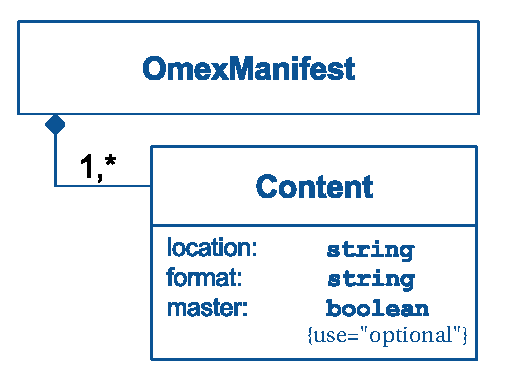
\includegraphics[width=6cm]{images/OmexManifest.pdf}\\
  \caption{A UML representation of the Manifest. Each manifest contains a number
	of Content elements.}
  \label{fig:combine_uml}
\end{figure}

\subsection{The \class{Content} class}
\label{content-class}
The \Content class represents an entry in the \OmexManifest and by 
extension a file in the \textit{COMBINE archive}. It consists of two 
required attributes: \token{location} and \token{format} and the 
optional attribute \token{master} 

\paragraph{The \token{location} attribute}
The \token{location} attribute is a required attribute of type 
\token{string}. It represents a relative location to an entry within the 
archive. The archive is represented by a dot \token{'.'}. 

\paragraph{The \token{format} attribute}
The \token{format} attribute is a required attribute of type \token{string}. It 
indicates the file type of the \Content element. The allowed values of the 
\token{format} attribute fall in two categories. Either the format 
denotes one of the COMBINE standards, in which case the \token{format} 
will begin with its \token{identifiers.org} URI. Or the 
\token{format} will represent a MIME type, in which case the \token{format} 
will begin with its \token{purl.org} URI. 

Using \token{identifiers.org} URI allows to unambiguously define the COMBINE standard, and even its level and version. For example, the identifier: \token{http://identifiers.org/combine.specifications/sbml} would denote the \Content 
element as being encoded in the SBML format. That is usually sufficient, as tools supporting one level of SBML usually
support others as well. However, if the software exporting the COMBINE archive wanted to be more precise, it could specify that it is an SBML Level 2 document with 

\begin{center}
\token{http://identifiers.org/combine.specifications/sbml.level-2}
\end{center}

or even declare its Version with 

\begin{center}
\token{http://identifiers.org/combine.specifications/sbml.level-2.version-3}.
\end{center}

The MIME type \token{purl.org} URI would be of the form \token{http://purl.org/NET/mediatypes/}
followed by the MIME type. Here are a few examples :

\begin{example}
    http://purl.org/NET/mediatypes/image/png
    http://purl.org/NET/mediatypes/application/pdf
    http://purl.org/NET/mediatypes/application/sbml+xml
\end{example}

If both an \token{identifiers.org} URI and a MIME type are available for one specific format, you should use the
\token{identifiers.org} URI. 

For compatibility reason, when reading a manifest.xml, you should be able to read format
attribute that contain only the MIME type, not in it's URI form. That is due to the fact that the draft specification
was allowing to use directly the MIME type for some time and some COMBINE archive using this form could be encountered.
However, when creating a new COMBINE archive, the URI form should always be used for MIME type.

\paragraph{The \token{master} attribute}
\label{active_document}
The \token{master} attribute is an optional attribute of type \token{boolean}. It 
represents a hint, that a certain file is to be used first when 
processing the content of an archive. Are top model description in a 
composed model, calling the various submodels; simulation description, 
calling the different model descriptions and data sources used in the 
experiment. In most cases, one content element per archive will have its \token{master} 
attribute set to \token{true}.

For example in the snippet below, it is the 
SED-ML element with \token{location="simulation.xml"} that a software 
program should first present to their users.

\begin{example}
<?xml version="1.0" encoding="utf-8"?>
<omexManifest xmlns="http://identifiers.org/combine.specifications/omex-manifest">
    <content location="." format="http://identifiers.org/combine.specifications/omex"/>
    <content location="manifest.xml" 
        format="http://identifiers.org/combine.specifications/omex-manifest"/>
    <content location="model/model.xml" format="http://identifiers.org/combine.specifications/sbml"/>
    <content location="simulation.xml" master="true"
        format="http://identifiers.org/combine.specifications/sedml"/>
    <content location="./article.pdf" format="http://purl.org/NET/mediatypes/application/pdf"/>
    <content location="./metadata.rdf"
        format="http://identifiers.org/combine.specifications/omex-metadata"/>
    <content location="diagram.sbgn" format="http://identifiers.org/combine.specifications/sbgn"/>
</omexManifest>
\end{example}

To simplify the identification, by a user or software, of the active document inside an archive, the file extensions 
(see also \ref{combine-archive-extensions}) can also be used. For the example above, 
where a SED-ML document is being marked as the master document, the 
recommended extension would be \token{.sbex}, to indicate that the software reading the archive need
to support the \token{SBML} format to be able to interpret the content of the archive. If the software
does support SED-ML as well as SBML, it should load the SED-ML file as the creator of the archive indicated
it to be the '\token{master}' file. If the software doesn't support SED-ML, it can still open the SBML document, ignoring
the master attribute.

Alternatively, if a software doesn't support either SBML or SED-ML but can open one of the other files, like the pdf
or diagram describing the model, it can choose to disregard the \token{master} attribute and the archive extension to present to the user the
files that it support.

In some cases, the \token{master} attribute could appear to be a duplication of the information given by the archive file
extension. But in other cases, like the example below, the \token{master} attribute add some usefull information.


\begin{example}
<?xml version="1.0" encoding="utf-8"?>
<omexManifest xmlns="http://identifiers.org/combine.specifications/omex-manifest">
    <content location="." format="http://identifiers.org/combine.specifications/omex"/>
    <content location="manifest.xml" 
        format="http://identifiers.org/combine.specifications/omex-manifest"/>
    <content location="main-model.xml" master=true 
        format="http://identifiers.org/combine.specifications/cellml.1.1"/>
    <content location="submodel1.xml" 
        format="http://identifiers.org/combine.specifications/cellml.1.1"/>
    <content location="submodel2.xml" 
        format="http://identifiers.org/combine.specifications/cellml.1.1"/>
    <content location="article.pdf" format="http://purl.org/NET/mediatypes/application/pdf"/>
    <content location="metadata.rdf"
        format="http://identifiers.org/combine.specifications/omex-metadata"/>
</omexManifest>
\end{example}

The archive, described by this manifest.xml, contain a modular CellML model. Even if the extension of the archive is \token{cmex}, it
does not help knowing which file to open first since there are several CellML files. The \token{master} attribute allow the software
to know which file encode the whole model.


\subsection{Advised format for the archive metadata}

One can include any type of file in a COMBINE archive, and therefore any 
type of metadata format. However, in the interest of interoperability, 
and to ease the development of software support for metadata, a 
recommended format is provided as part of the specification of the 
archive. 

The recommended format is based on several standards developed by other 
organisations: 

\begin{itemize}
	\item  {
	
     The \href{http://www.w3.org/RDF/ }{ Resource Description Format} of the 
     W3C, in particular its terms:
     \begin{itemize}
		\item \token{RDF}, 
		\item \token{Description}, 
		\item \token{Bag}, 
		\item \token{li}.
	\end{itemize}
	}
	\item  {

	vCard 4 (\cite{rfc6350}), a file format standard for electronic business 
    cards, in particular its terms:
    	\begin{itemize}
		\item \token{hasName}, 
		\item \token{family-name}, 
		\item \token{given-name}, 
		\item \token{hasEmail},
		\item \token{organization-name}.
	\end{itemize}

	More information on how to use vCard in RDF can be found 
    on the W3C website\footnote[1]{\url{http://www.w3.org/TR/vcard-rdf/ }}.
	
	}
	\item {
	
	Metadata terms\footnote[2]{\url{http://dublincore.org/documents/dcmi-terms/}} of 
	the Dublin Core Metadata Initiative, in particular the terms: 

	\begin{itemize}
		\item \token{description}, 
		\item \token{creator}, 
		\item \token{created}, 
		\item \token{modified},
		\item \token{W3CDTF}.
	\end{itemize}
		
	More information on the use of Dublin Core in RDF can be found 
	on the Dublin Core website{\footnote[3]{\url{http://dublincore.org/documents/dc-rdf/}}}. } 
	
	More information is available about the definition of the date format used within \token{dcterms:created} and 
	\token{dcterms:modified} elements{\footnote[4]{\url{http://www.w3.org/TR/NOTE-datetime}}}.

\end{itemize}
\pagebreak
Users of the COMBINE standards may already be familiar with this 
approach, as it is also taken by the Systems Biology Markup Language. 
Note however that the format here slightly differs from the controlled 
annotations of SBML. The differences have been made to address inconsistencies 
in the SBML vCard specification and to follow W3C recommendations {\footnote[4]{\url{http://www.w3.org/TR/vcard-rdf/}}} . The changes 
are:

\begin{itemize}
	\item  "n" becomes "hasName" 
	\item  "Family" becomes "family-name" 
	\item  "Given" becomes "given-name" 
	\item  "EMAIL" becomes "hasEmail" 
	\item  "Orgname" becomes "organization-name" 
\end{itemize}

A \textit{COMBINE archive} can include multiple metadata elements. To 
identify that a particular \Content element is being annotated, the 
\token{rdf:about} attribute should use the same value that is also used 
in \token{location} of the \Content element. 


\begin{example}
<?xml version="1.0" encoding="UTF-8"?>
<rdf:RDF xmlns:rdf="http://www.w3.org/1999/02/22-rdf-syntax-ns#" 
         xmlns:dcterms="http://purl.org/dc/terms/" 
				 xmlns:vCard="http://www.w3.org/2006/vcard/ns#">
   <rdf:Description rdf:about="./simulation.xml">
   ...
	 </rdf:Description>
</rdf:RDF>
\end{example}

The example above signifies that a content element with 
\token{location="./simulation.xml"} is described. A complete example of 
the metadata related to a simulation description contained in a COMBINE 
archive is described in \ref{examples}. 


